% =================== PAGE DE GARDE ===================
% Pour ajouter les membres de l'équipe : modifier la ligne « \newcommand{\equipe}{...} » ci-dessous.
\newcommand{\equipe}{Farah Belghith}
\begin{titlepage}
\newgeometry{top=1.4cm,bottom=1.6cm,left=2.4cm,right=2.4cm}
\setstretch{1.05}
\centering
\noindent
\begin{minipage}[c]{0.3\linewidth}\raggedright
  
\includegraphics[height=2.1cm,keepaspectratio]{figures/logo_univ_tunis.png}
\end{minipage}%
\begin{minipage}[c]{0.4\linewidth}\centering
  
\includegraphics[height=2.2cm,keepaspectratio]{figures/logo_emblem.png}
\end{minipage}%
\begin{minipage}[c]{0.3\linewidth}\raggedleft
  
\includegraphics[height=1.5cm,keepaspectratio]{figures/logo_ensit.png}
\end{minipage}

\vspace{0.5cm}
\rule{\linewidth}{1pt}\par
\vspace{0.35cm}
{\large\bfseries UNIVERSITÉ DE TUNIS\par}
\vspace{2pt}
{\large\bfseries ÉCOLE NATIONALE SUPÉRIEURE D'INGÉNIEURS DE TUNIS\par}
\vspace{2pt}
{\bfseries DÉPARTEMENT DE GÉNIE MATHÉMATIQUE\par}
\vspace{0.3cm}
\rule{\linewidth}{1pt}\par

\vfill
{\LARGE\bfseries Projet de Sûreté de Fonctionnement et Maintenance\par}
\vspace{0.35em}
{\normalsize\bfseries Troisième année — Génie Mathématiques Appliquées et Modélisation (GMAM 3)\par}

\vspace{0.7cm}
{\normalsize Réalisé par :\par}
\vspace{0.4em}
{\LARGE\bfseries \equipe\par}

\vfill
{\color{terre}\rule{0.85\linewidth}{0.8pt}}\par
\vspace{0.7em}
{\fontsize{24}{30}\selectfont\bfseries Étude comparative de pronostic\\ de défaillance de roulements\par}
\vspace{0.5em}
{\large\bfseries Fiabilité, premier défaut, durée de vie résiduelle\\ et décision de maintenance (FEMTO-ST / PRONOSTIA)\par}
\vspace{0.7em}
{\color{terre}\rule{0.85\linewidth}{0.8pt}}\par

\vfill
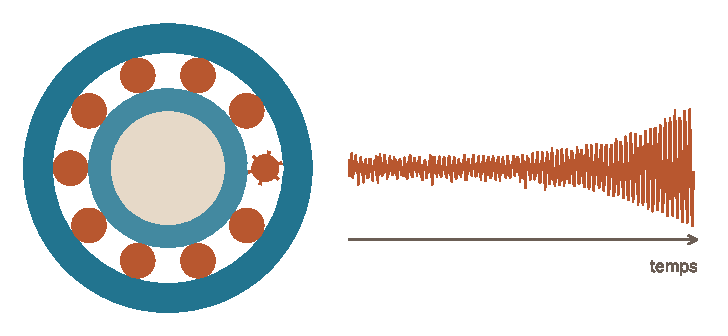
\includegraphics[height=3.9cm,keepaspectratio]{figures/illustration_couverture.pdf}\par

\vfill
{\normalsize Rapport de projet\par}
\vspace{0.5em}
{\normalsize\textbf{Encadré par :} M. Fayçal Ben Hmida\par}

\vfill
{\normalsize\textbf{Année universitaire :} 2026–2027\par}

\restoregeometry
\end{titlepage}
